\begin{frame}{CFD Process Simulation Flow Chart}
    \begin{figure}
    \centering
    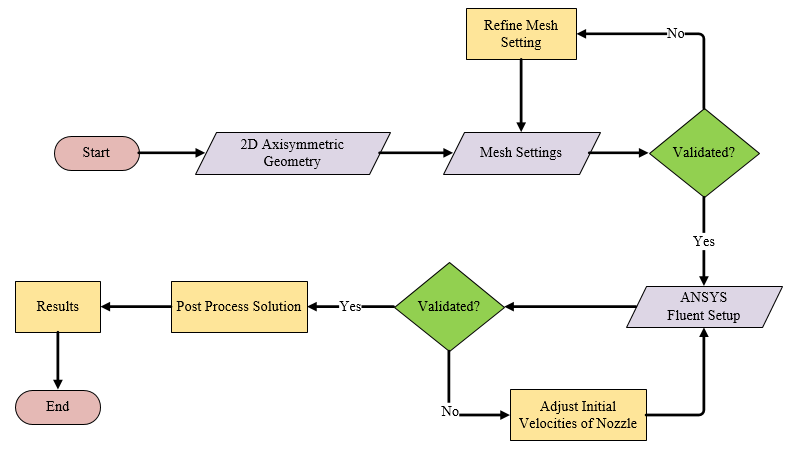
\includegraphics[height=0.45\textwidth]{images/SimulationProcessFlowChart.PNG}
    \label{fig:ejectorprocessflowchart}
\end{figure}
\end{frame}

\begin{frame}{2D Axisymmetric Model}
  \begin{figure}[h]
    \centering
    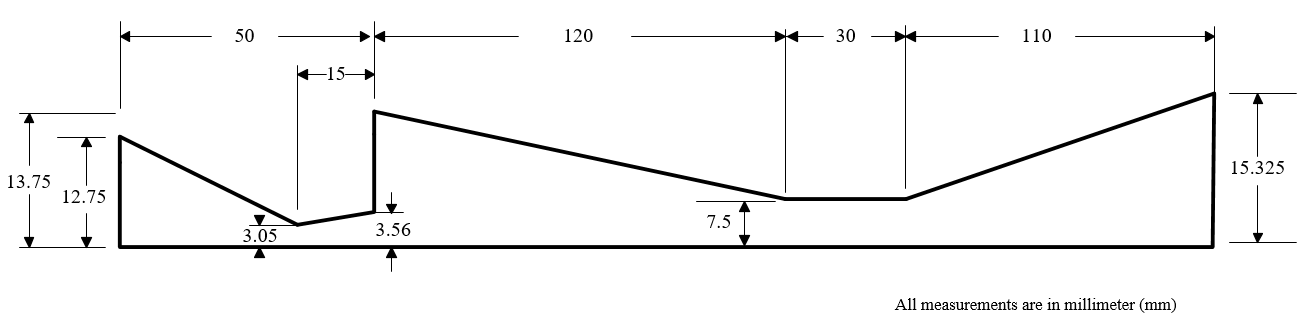
\includegraphics[width=1\textwidth]{images/ejectordrawing.png}
    \caption{Two Dimensional Axisymmetric Drawing of Ejector based from the 3D Geometry of Shah et al.\cite{shah2014experimental}}
    \label{fig:2daxisymmetricejector}
 \end{figure}
\end{frame}

\begin{frame}{Mesh Settings}
   \begin{figure}[h]
    \centering
    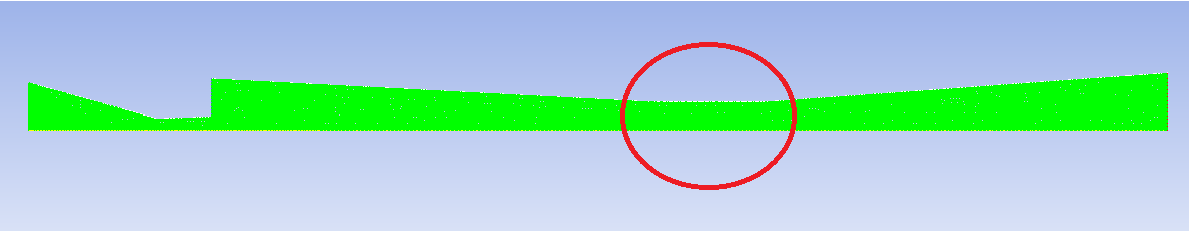
\includegraphics[width=0.5\textwidth]{images/Meshemphasized.png}
    \label{fig:meshrefinement1}
  \end{figure}
  \begin{table}[h]
      \centering
       \caption{Number of Elements and Nodes for Each Mesh Settings}
      \label{tab:meshelementsandnodes}
      \begin{tabular}{ccc}
      \hline
         Mesh Settings  &  Elements & Nodes\\
      \hline
         Refinement Level 1  & 87,412 & 178,106 \\
         Refinement Level 2 & 196,620 & 398,162 \\
         Refinement Level 3 & 349,496 & 705,554 \\
         Refinement Level 4 & 539,716 & 1,087,722 \\
      \hline
      \end{tabular}
  \end{table}
\end{frame}

\begin{frame}{Mesh Settings: Refinement Level 1}
  \begin{figure}[h]
    \centering
    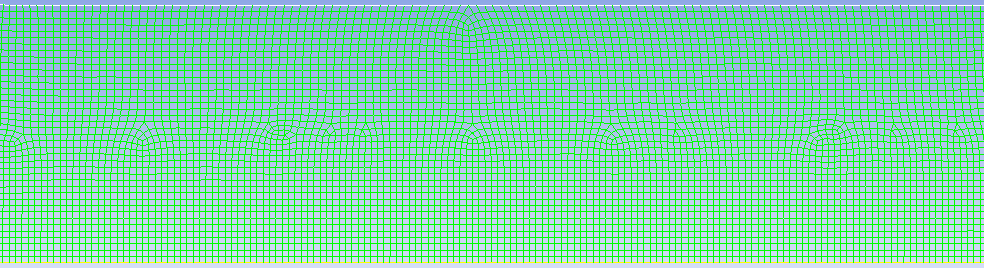
\includegraphics[width=1\textwidth]{images/MeshRef1.png}
    \label{fig:meshrefinement1}
  \end{figure}
\end{frame}

\begin{frame}{Mesh Settings: Refinement Level 2}
    \begin{figure}[h]
    \centering
    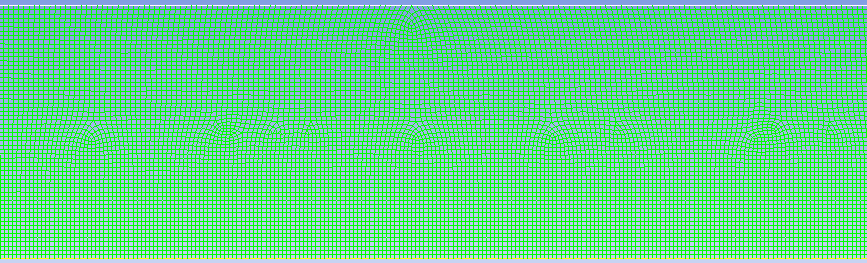
\includegraphics[width=1\textwidth]{images/MeshRef2.png}
    \label{fig:meshrefinement2}
  \end{figure}
\end{frame}

\begin{frame}{Mesh Settings: Refinement Level 3}
    \begin{figure}[h]
    \centering
    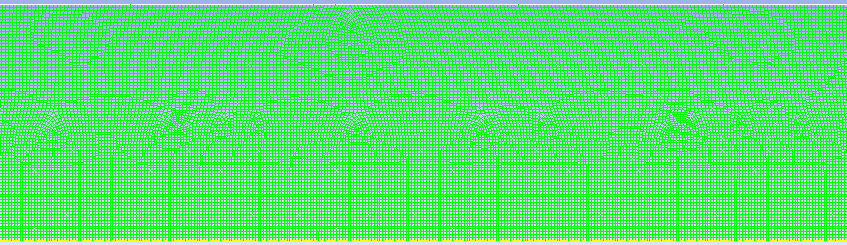
\includegraphics[width=1\textwidth]{images/MeshRef3.PNG}
    \label{fig:meshrefinement3}
  \end{figure}
\end{frame}

\begin{frame}{Mesh Settings: Refinement Level 4}
    \begin{figure}[h]
    \centering
    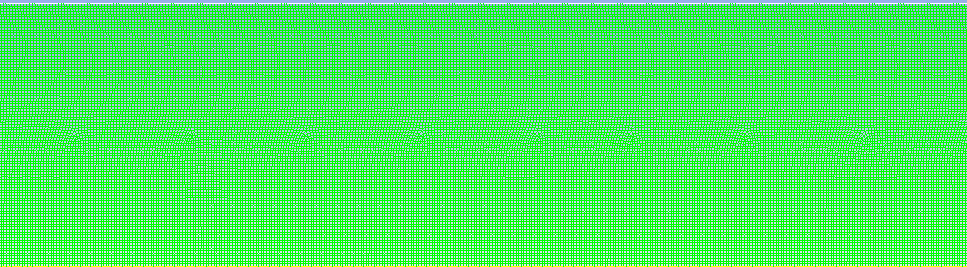
\includegraphics[width=1\textwidth]{images/MeshRef4.PNG}
    \label{fig:meshrefinement4}
  \end{figure}
\end{frame}

\begin{frame}{Mesh Metrics and Computational Time}
    \begin{table}[h]
      \centering
       \caption{Mesh Metrics and Computational Time for Each Mesh Settings}
      \label{tab:meshelementsandnodes}
      \begin{tabular}{cccc}
      \hline
         Mesh Settings  & Orthogonal Quality  & Min. Aspect Ratio & Solving Time\\
      \hline
         Ref. Level 1  & 0.764862 & 3.32878 & 15 hours\\
         Ref. Level 2 & 0.751712 & 3.54955 & 70 hours\\
         Ref. Level 3 & 0.712621 & 3.48676 & 120 hours\\
         Ref. Level 4 & 0.816016 & 3.22583 & 170 hours\\
      \hline
      \end{tabular}
  \end{table}
\end{frame}

\begin{frame}{Mesh Independent Study:Static Pressure of the Mixture}
    \begin{figure}[h]
      \centering
      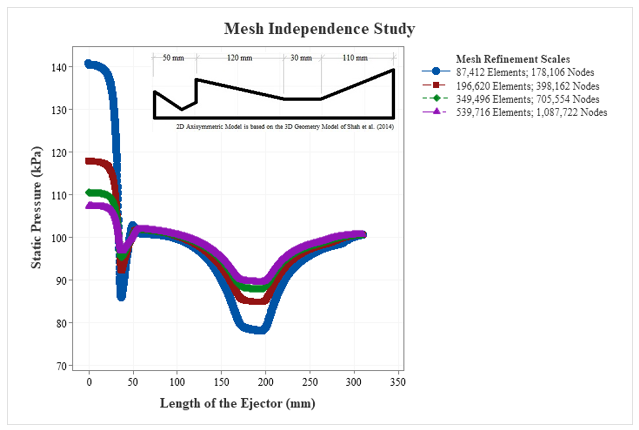
\includegraphics[height=5cm]{images/MISstaticpressure.png}
      \label{fig:meshindependentstudy}
   \end{figure}
\end{frame}

\begin{frame}{Mesh Independent Study: Pressure Coefficient and the Total Pressure}
    \begin{columns}
      \column{0.45\textwidth}
      \begin{figure}[h]
      \centering
      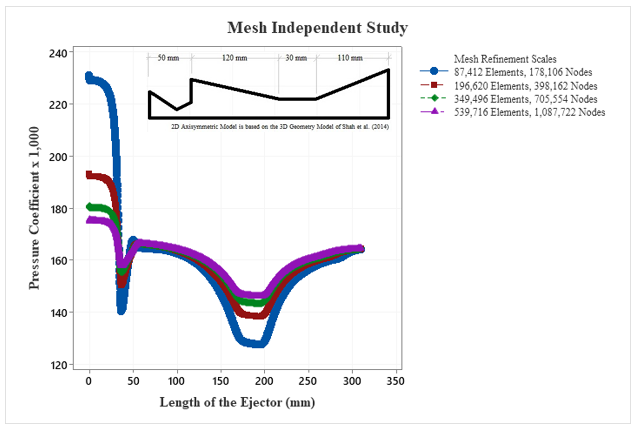
\includegraphics[height=4.5cm]{images/MISPCcalibrated.png}
      \label{fig:meshindependentstudy}
      \end{figure}
      \column{0.45\textwidth}
      \begin{figure}[h]
      \centering
      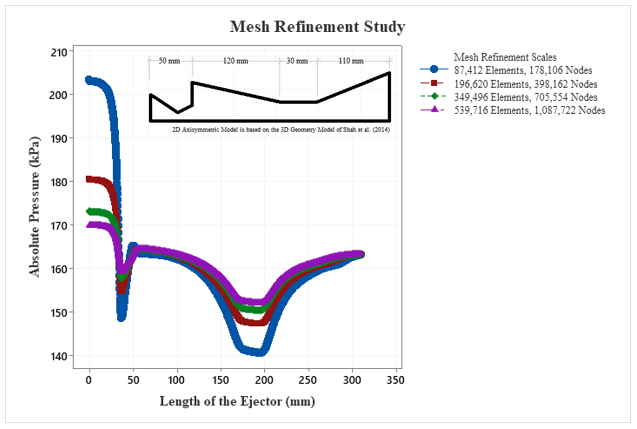
\includegraphics[height=4.5cm]{images/MISAbsP.png}
      \label{fig:meshindependentstudy}
      \end{figure}
    \end{columns}
\end{frame}

\begin{frame}{Mesh Independent Study: Dynamic Pressure}
       \begin{columns}
      \column{0.45\textwidth}
      \begin{figure}[h]
      \centering
      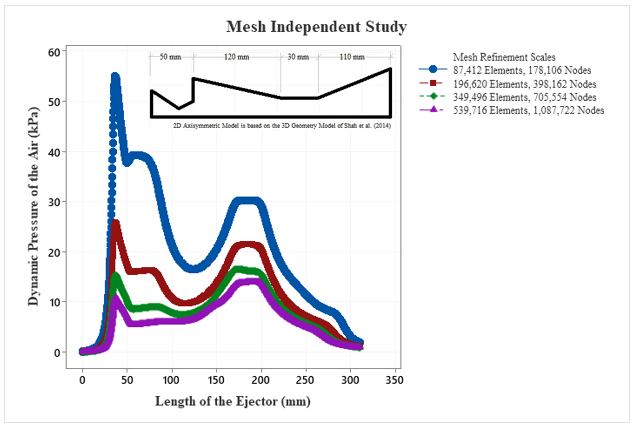
\includegraphics[height=4.5cm]{images/MISdynapair.png}
      \label{fig:meshindependentstudy}
      \end{figure}
      \column{0.45\textwidth}
      \begin{figure}[h]
      \centering
      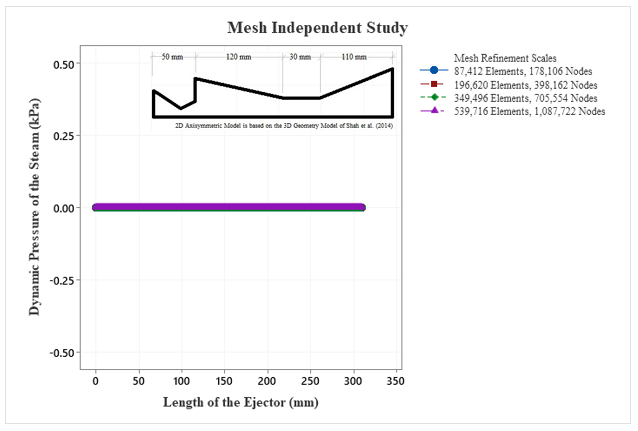
\includegraphics[height=4.5cm]{images/MISdynapsteam.png}
      \label{fig:meshindependentstudy}
      \end{figure}
    \end{columns}
\end{frame}

\begin{frame}{Mesh Independent Study: Dynamic Pressure}
       \begin{columns}
      \column{0.45\textwidth}
      \begin{figure}[h]
      \centering
      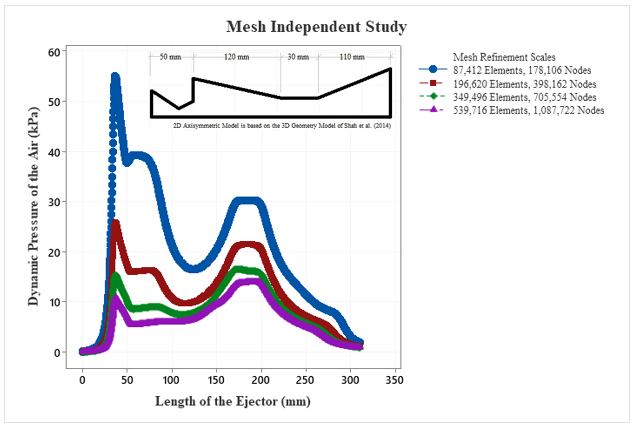
\includegraphics[height=4.5cm]{images/MISdynapair.png}
      \label{fig:meshindependentstudy}
      \end{figure}
      \column{0.45\textwidth}
      \begin{figure}[h]
      \centering
      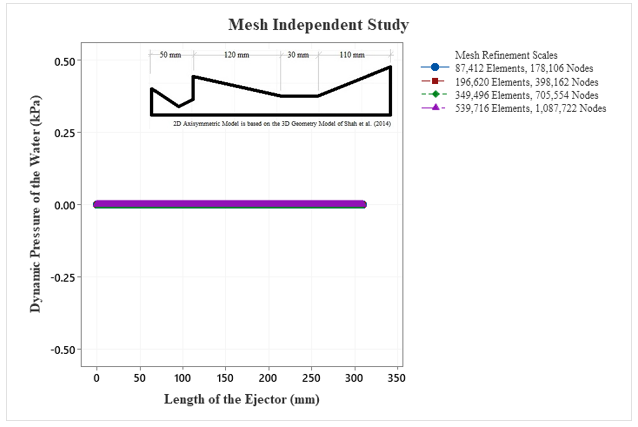
\includegraphics[height=4.5cm]{images/MISdynapwater.png}
      \label{fig:meshindependentstudy}
      \end{figure}
    \end{columns}
\end{frame}

\begin{frame}{Mesh Independent Study: Relative Total Pressure}
       \begin{columns}
      \column{0.45\textwidth}
      \begin{figure}[h]
      \centering
      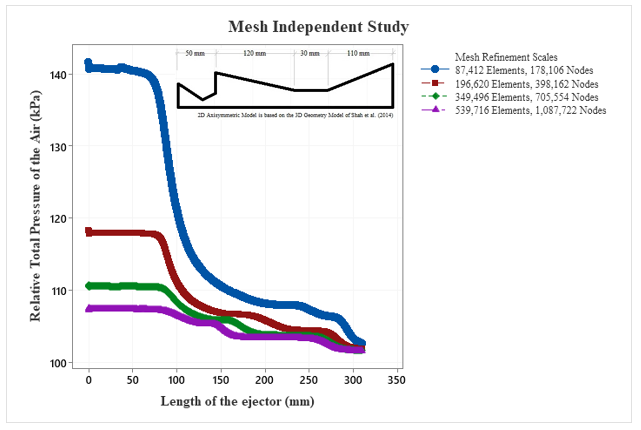
\includegraphics[height=4.5cm]{images/MISRelTPAir.png}
      \label{fig:meshindependentstudy}
      \end{figure}
      \column{0.45\textwidth}
      \begin{figure}[h]
      \centering
      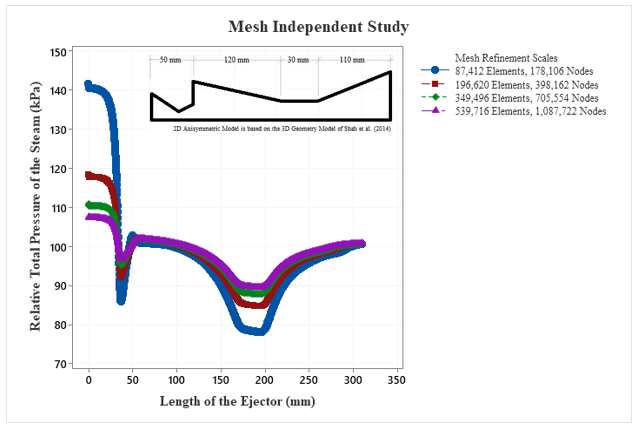
\includegraphics[height=4.5cm]{images/MISRTPsteam.png}
      \label{fig:meshindependentstudy}
      \end{figure}
    \end{columns}
\end{frame}

\begin{frame}{Mesh Independent Study: Relative Total Pressure}
       \begin{columns}
      \column{0.45\textwidth}
      \begin{figure}[h]
      \centering
      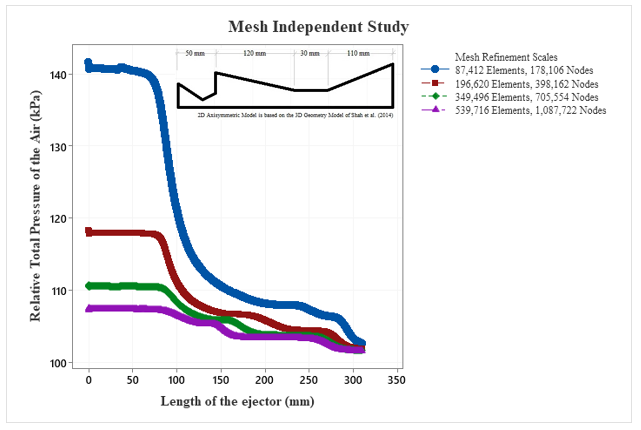
\includegraphics[height=4.5cm]{images/MISRelTPAir.png}
      \label{fig:meshindependentstudy}
      \end{figure}
      \column{0.45\textwidth}
      \begin{figure}[h]
      \centering
      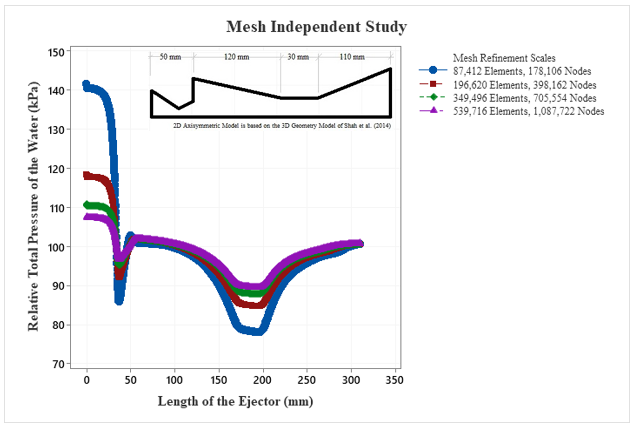
\includegraphics[height=4.5cm]{images/MISRelTPwater.png}
      \label{fig:meshindependentstudy}
      \end{figure}
    \end{columns}
\end{frame}

\begin{frame}{Mesh Independent Study: Total Pressure}
       \begin{columns}
      \column{0.45\textwidth}
      \begin{figure}[h]
      \centering
      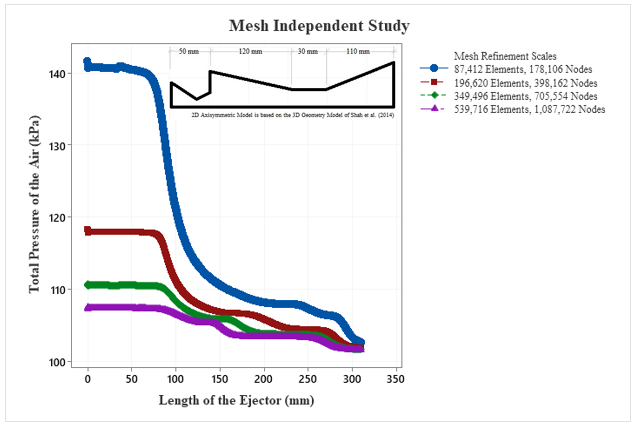
\includegraphics[height=4.5cm]{images/MISTPAir.png}
      \label{fig:meshindependentstudy}
      \end{figure}
      \column{0.45\textwidth}
      \begin{figure}[h]
      \centering
      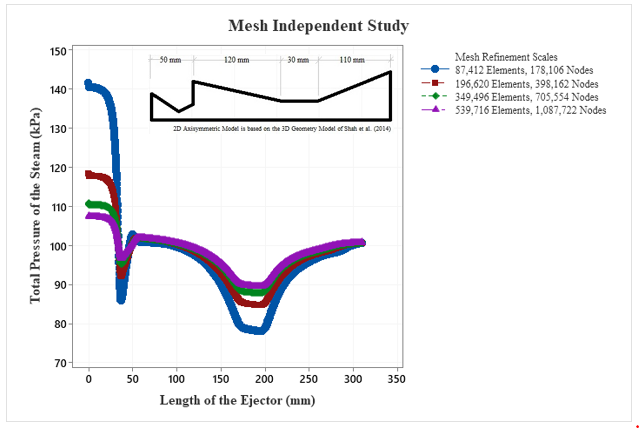
\includegraphics[height=4.5cm]{images/MISTPsteam.png}
      \label{fig:meshindependentstudy}
      \end{figure}
    \end{columns}
\end{frame}

\begin{frame}{Mesh Independent Study: Total Pressure}
       \begin{columns}
      \column{0.45\textwidth}
      \begin{figure}[h]
      \centering
      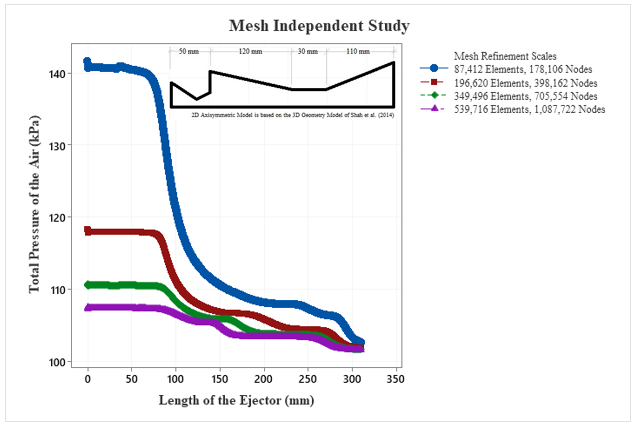
\includegraphics[height=4.5cm]{images/MISTPAir.png}
      \label{fig:meshindependentstudy}
      \end{figure}
      \column{0.45\textwidth}
      \begin{figure}[h]
      \centering
      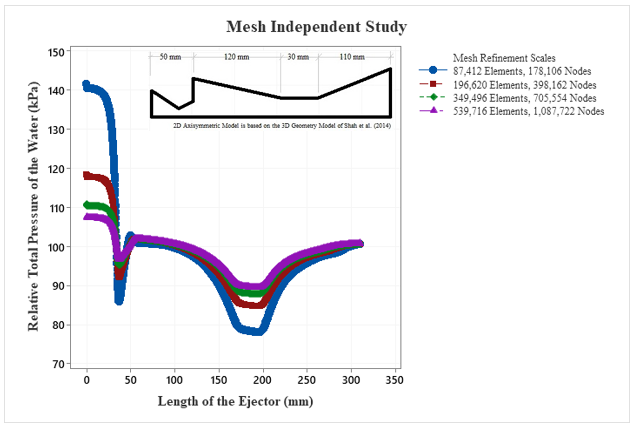
\includegraphics[height=4.5cm]{images/MISRelTPwater.png}
      \label{fig:meshindependentstudy}
      \end{figure}
    \end{columns}
\end{frame}

\begin{frame}{Computational Domain of the 2D Axisymmetric Ejector}
    \begin{table}[h]
    \centering
    \caption{Computational Domain of the 2D Axisymmetric Ejector using Refinement Level 3}
    \label{tab:computationaldomainejector}
    \begin{tabular}{ccc}
    \hline
        Domain Extents & Minimum (mm) & Maximum (mm) \\
    \hline
        x-coordinate &  -64.6339 & 245.3661 \\
        y-coordinate & 0.0000 & 15.325 \\
    \hline
    \end{tabular}
\end{table}
\end{frame}

\begin{frame}{Volume and Face Area Statistics of the 2D Axisymmetric Ejector using Refinement Level 3}
\begin{table}[h]
    \centering
    \caption{Volume Statistics}
    \label{tab:volumestat}
    \begin{tabular}{|c|c|}
      \hline
        Minimum volume (mm\textsuperscript3) &  0.002245853\\
     \hline
        Maximum volume (mm\textsuperscript3) & 0.8284871\\
     \hline
        Total volume (mm\textsuperscript3) & 104,100.4 \\
     \hline
        Minimum 2d volume (mm\textsuperscript3) & 2.593306 \\
     \hline
        Maximum 2d volume (mm\textsuperscript3) & 15.79421 \\
     \hline
    \end{tabular}
\end{table}
\begin{table}[h]
    \centering
    \caption{Face Area Statistics}
    \label{tab:faceareastat}
    \begin{tabular}{|c|c|}
       \hline
        Minimum face area (mm\textsuperscript2) & 50.53009  \\
       \hline
        Maximum face area (mm\textsuperscript2) & 162.0518 \\
       \hline
    \end{tabular}
\end{table}
\end{frame}

\begin{frame}{Material Properties: Stainless Steel AISI316}
    \begin{table}[h]
        \centering
        \begin{tabular}{|c|c|}
        \hline
            Density & 8,000 kg/m\textsuperscript{3} \\
        \hline
            Specific Heat & 500 J/kg K \\
        \hline
            Thermal Conductivity & 16.3 W/m K \\
        \hline
        \end{tabular}
        \label{tab:steelaiai316}
    \end{table}
\end{frame}
\begin{frame}{Fluid Properties: Steam Central Jet}
    \begin{table}[h]
        \centering
        \caption{Properties of Air}
        \label{tab:airprop}
        \begin{tabular}{|c|c|}
        \hline
            Density & 1.225 kg/m\textsuperscript{3}\\
        \hline
            Specific Heat & 1,006.43 J/kg K \\
        \hline
            Thermal Conductivity & 0.0242 W/m K \\
        \hline
            Viscosity & 1.7894e-05 kg/m-s \\
        \hline
            Molecular Weight & 28.966 kg/kmol \\
        \hline
            Standard State Enthalpy & 0 J/kg mol \\
        \hline
            Reference Temperature & 298.15 K \\
        \hline
        \end{tabular}
    \end{table}
\end{frame}

\begin{frame}{Fluid Properties: Steam Central Jet}
    \begin{table}[h]
        \centering
        \caption{Properties of Steam}
        \label{tab:steamprop}
        \begin{tabular}{|c|p{3cm}|}
        \hline
            Density  & $\rho = -31.14307 + 0.3099722 T - 0.00103197 T^{2} + 1.15e-06 T^{3}$\\
        \hline
            Specific Heat &  2121 J/kg K \\
        \hline
            Thermal Conductivity & 0.025506 W/m K \\
        \hline
            Viscosity & 1.2555e-05 kg/m-s \\
        \hline
            Molecular Weight & 18.01534 kg/kmol \\
        \hline
            Standard State Enthalpy & -2.418379e+08 J/kg mol \\
        \hline
            Reference Temperature & 298.15 K \\
        \hline
        \end{tabular}
    \end{table}
    Density varies from 280 to 400 K.
\end{frame}

\begin{frame}{Fluid Properties: Steam Central Jet}
    \begin{table}[h]
        \centering
        \caption{Properties of Water}
        \label{tab:waterprop}
        \begin{tabular}{|c|c|}
        \hline
            Density  & 998.8 kg/m\textsuperscript{3}\\
        \hline
            Specific Heat &  4186.6 J/kg K \\
        \hline
            Thermal Conductivity & 0.59229 W/m K \\
        \hline
            Viscosity & 0.001084 kg/m-s \\
        \hline
            Molecular Weight & 18.01534 kg/kmol \\
        \hline
            Standard State Enthalpy & -2.858412e+08 J/kg mol \\
        \hline
            Reference Temperature & 298.15 K \\
        \hline
        \end{tabular}
    \end{table}
\end{frame}

\begin{frame}{Boundary Conditions: Steam Central Jet}
\begin{table}[h]
    \centering
    \caption{Ejector Inlet Conditions}
    \label{tab:ejectorbc}
    \begin{tabular}{|c|c|}
    \hline
        Ejector & Water Inlet \\
    \hline
        Pressure Inlet & 93.56 kPa \\
    \hline
        Temperature Inlet & 290 K \\
    \hline
        Inlet Velocity & 31.73435 m/s \\
    \hline
    \end{tabular}
\end{table}
\begin{table}[h]
    \centering
    \caption{Nozzle Inlet Conditions}
    \label{tab:nozzlebc}
    \begin{tabular}{|c|c|}
    \hline
        Nozzle & Steam Inlet \\
    \hline
        Pressure Inlet & 140 kPa \\
    \hline
        Temperature Inlet & 382.44 K \\
    \hline
        Inlet Velocity & 0.75 m/s \\
    \hline
    \end{tabular}
\end{table}
\centering Ambient Pressure = 96 kPa
\end{frame}

\begin{frame}{Fluid Properties: Water Central Jet}
    \begin{table}[h]
        \centering
        \caption{Properties of Steam}
        \label{tab:steampropwcj}
        \begin{tabular}{|c|p{3cm}|}
        \hline
            Density  & $\rho = -7.6292 + 0.022047 T $\\
        \hline
            Specific Heat &  2071.1 J/kg K \\
        \hline
            Thermal Conductivity & 0.024352 W/m K \\
        \hline
            Viscosity & 1.2154e-05 kg/m-s \\
        \hline
            Molecular Weight & 18.01534 kg/kmol \\
        \hline
            Standard State Enthalpy & -2.418379e+08 J/kg mol \\
        \hline
            Reference Temperature & 298.15 K \\
        \hline
        \end{tabular}
    \end{table}
    Density varies from 370 to 385 K.
\end{frame}

\begin{frame}{Fluid Properties: Water Central Jet}
    \begin{table}[h]
        \centering
        \caption{Properties of Water}
        \label{tab:waterpropwcj}
        \begin{tabular}{|c|c|}
        \hline
            Density (Density varies from 370 to 385 K)  & $\rho = 1232.13 - 0.73368 T $\\
        \hline
            Specific Heat &  4227.4 J/kg K \\
        \hline
            Thermal Conductivity & 0.68017 W/m K \\
        \hline
            Viscosity & 0.00025636 kg/m-s \\
        \hline
            Molecular Weight & 18.01534 kg/kmol \\
        \hline
            Standard State Enthalpy & -2.858412e+08 J/kg mol \\
        \hline
            Reference Temperature & 298.15 K \\
        \hline
        \end{tabular}
    \end{table}
\end{frame}

\begin{frame}{CPU Specification}
    \begin{table}[]
        \centering
        \caption{Device Specification}
        \label{tab:devicespecification}
        \begin{tabular}{c|c}
            Processor &  Intel(R) Core(TM) i7-4700MQ CPU @ 2.40GHz   2.40 GHz\\
            Installed RAM & 16.0 GB (15.6 GB usable)\\
            System type & 64-bit operating system, x64-based processor \\
        \end{tabular}
    \end{table}
\end{frame}

\begin{frame}{CFD Models Used}
\begin{itemize}
    \item Eulerian Multiphase Model
    \item Explicit Volume Fraction Discretization
    \item Symmetric Model
    \item Two-Resistance Model
    \item Thermal-Phase Change Model
    \item Interfacial Area Concentration: Particle Method
    \item $\kappa-\varepsilon$ Realizable per Phase turbulence model
    \item Scalable Wall Function
\end{itemize}
\end{frame}

\begin{frame}{CFD Solution Methods and Controls}
    \begin{block}{Pressure-Velocity Coupling}
    Phase Coupled SIMPLE
    \end{block}
    \begin{block}{Spatial Discretization}
    Gradient Least Squares Cell Based
    \end{block}
    \begin{block}{Momentum, Turbulent Kinetic Energy, Turbulent Dissipation Rate and Energy}
    QUICK Scheme
    \end{block}
    \begin{block}{Volume Fraction}
    Modified HRIC
    \end{block}
\end{frame}

\begin{frame}{CFD Solution Monitors: Residual Errors}
  \begin{columns}
    \column{0.45\textwidth}
    \begin{table}[h]
        \centering
        \begin{tabular}{cc}
        \hline
            Residuals & Convergence Criterion \\
        \hline
            Continuity & 1e-08\\
            u-air & 1e-08\\
            u-steam & 1e-08\\
            u-water & 1e-08\\
            v-air & 1e-08\\
            v-steam & 1e-08\\
            v-water & 1e-08\\
        \hline
        \end{tabular}
    \end{table}
    \column{0.45\textwidth}
    \begin{table}[h]
        \centering
        \begin{tabular}{cc}
        \hline
            Residuals & Convergence Criterion \\
        \hline
            energy-p1 & 1e-08\\
            energy-p2 & 1e-08\\
            energy-p3 & 1e-08\\
            k-air & 1e-08\\
            k-steam & 1e-08\\
            k-water & 1e-08\\
            eps-air & 1e-08\\
            eps-steam & 1e-08\\
            eps-water & 1e-08\\
        \hline
        \end{tabular}
    \end{table}
  \end{columns}
\end{frame}